\documentclass[tikz,border=8pt]{standalone}
% Shared look for every TikZ diagram. Load with \input{../../tools/tikz-style.tex}
\usepackage[T1]{fontenc}
\usepackage{lmodern}
\renewcommand{\sfdefault}{lmr}  % diagrams use the same serif as the text
\usetikzlibrary{arrows.meta, positioning, shapes.geometric, calc, fit, backgrounds}
\definecolor{cblue}{HTML}{4C78A8}
\definecolor{corange}{HTML}{F58518}
\definecolor{cgreen}{HTML}{54A24B}
\definecolor{cred}{HTML}{E45756}
\definecolor{cpurple}{HTML}{B279A2}
\definecolor{cgrey}{HTML}{6B6B6B}
\tikzset{
  every picture/.style={font=\sffamily, line width=1.2pt},
  box/.style={draw=#1, fill=#1!12, rounded corners=4pt, align=center, inner sep=7pt, minimum height=1.1cm},
  box/.default=cgrey,
  arrow/.style={-{Stealth[length=3mm]}, draw=cgrey, line width=1.4pt},
  title/.style={font=\sffamily\bfseries\Large},
  note/.style={font=\sffamily\small, text=cgrey, align=center},
}
\AtBeginDocument{\hyphenpenalty=10000 \exhyphenpenalty=10000}

\begin{document}
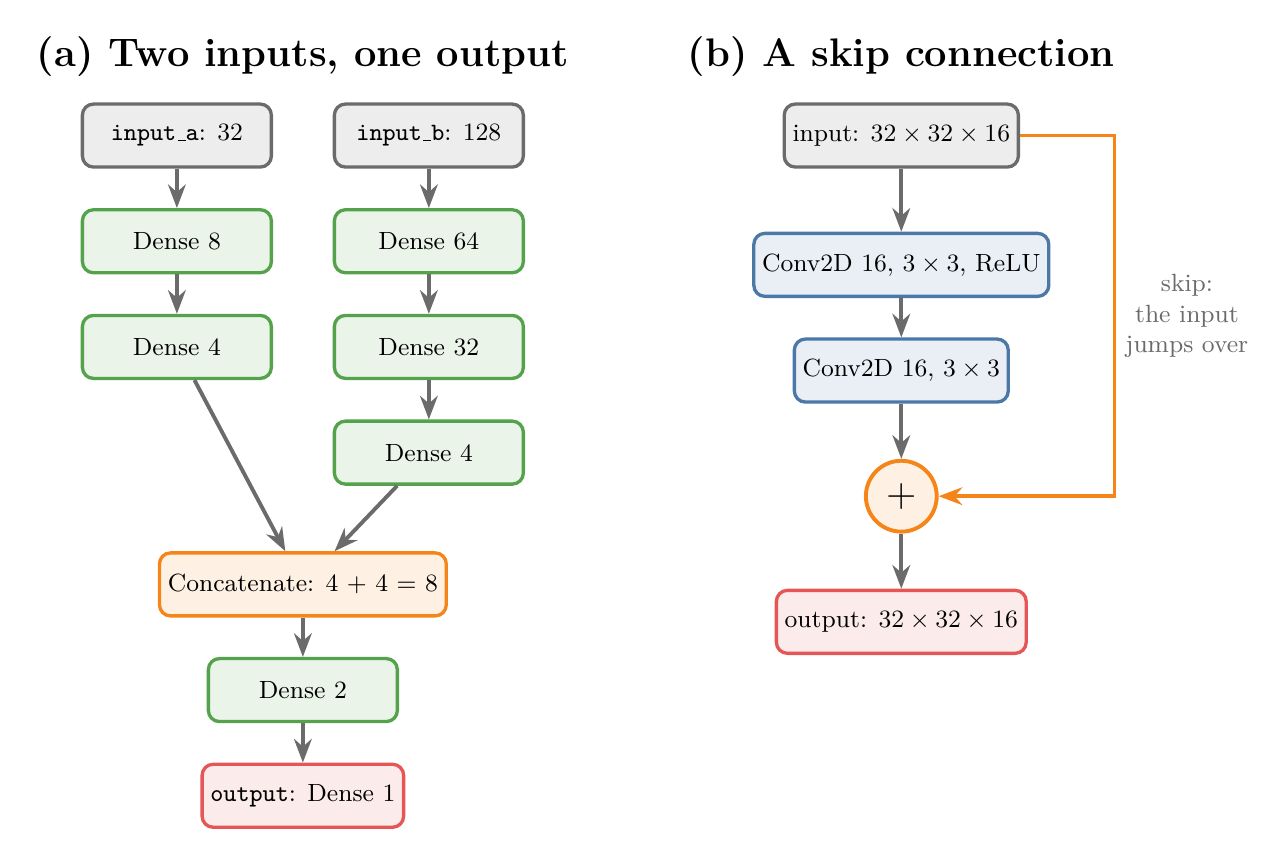
\begin{tikzpicture}[b/.style={box=#1, minimum width=2.4cm, minimum height=0.8cm, inner sep=3pt, font=\sffamily\small}, node distance=0.5cm]
  \begin{scope}
    \node[title] at (1.6, 1.0) {(a) Two inputs, one output};
    \node[b=cgrey] (a) at (0, 0) {\texttt{input\_a}: 32};
    \node[b=cgreen, below=of a] (a1) {Dense 8};
    \node[b=cgreen, below=of a1] (a2) {Dense 4};
    \node[b=cgrey] (b) at (3.2, 0) {\texttt{input\_b}: 128};
    \node[b=cgreen, below=of b] (b1) {Dense 64};
    \node[b=cgreen, below=of b1] (b2) {Dense 32};
    \node[b=cgreen, below=of b2] (b3) {Dense 4};
    \node[b=corange] (c) at (1.6, -5.7) {Concatenate: 4 + 4 = 8};
    \node[b=cgreen, below=of c] (z) {Dense 2};
    \node[b=cred, below=of z] (out) {\texttt{output}: Dense 1};
    \draw[arrow] (a) -- (a1); \draw[arrow] (a1) -- (a2); \draw[arrow] (b) -- (b1); \draw[arrow] (b1) -- (b2); \draw[arrow] (b2) -- (b3);
    \draw[arrow] (a2) -- (c); \draw[arrow] (b3) -- (c); \draw[arrow] (c) -- (z); \draw[arrow] (z) -- (out);
  \end{scope}
  \begin{scope}[xshift=9.2cm]
    \node[title] at (0, 1.0) {(b) A skip connection};
    \node[b=cgrey] (i) at (0, 0) {input: $32 \times 32 \times 16$};
    \node[b=cblue, below=0.8cm of i] (c1) {Conv2D 16, $3 \times 3$, ReLU};
    \node[b=cblue, below=of c1] (c2) {Conv2D 16, $3 \times 3$};
    \node[circle, draw=corange, fill=corange!12, line width=1.4pt, minimum size=0.9cm, below=0.7cm of c2] (add) {\Large $+$};
    \node[b=cred, below=0.7cm of add] (o) {output: $32 \times 32 \times 16$};
    \draw[arrow] (i) -- (c1); \draw[arrow] (c1) -- (c2); \draw[arrow] (c2) -- (add); \draw[arrow] (add) -- (o);
    \draw[arrow, draw=corange] (i.east) -- ++(1.2, 0) |- (add.east) node[pos=0.25, right, note] {skip:\\the input\\jumps over};
  \end{scope}
\end{tikzpicture}
\end{document}
